\section{Paradigma Funcional}
\begin{frame}{Introdução a programação funcional}
	\begin{block}{Entidades de primeira-classe}
	\begin{itemize}
		\item Entidades que podem ser passadas como parâmetro
		\item Podem ser retornadas como resultado
		\item Podem ser armazenadas em estruturas de dados
	\end{itemize}
	\end{block}
\end{frame}
\begin{frame}{A Programação Funcional}
	\begin{block}{Modelo computacional}
		\begin{itemize}
			\item Função de x em y : Mapeamento de valores de entrada em valores de saída
			\item Ausência de estado e comandos (atribuição + controle)
		\end{itemize}		
	\end{block}
	\begin{center}
		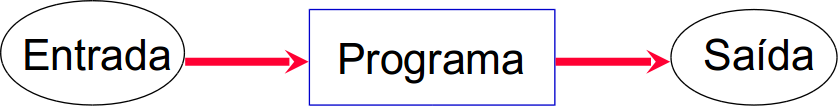
\includegraphics[scale=0.3]{paradigma_funcional/modelo_funcional.png}
	\end{center}
\end{frame}
\begin{frame}{Paradigma Funcional}
	\begin{block}{Mudando o foco}
		\begin{itemize}
			\item sem laços?
			\item sem efeitos colaterais?
			\item sem mudar o valor de variáveis?
		\end{itemize}
	\end{block}
	\begin{block}{Aplicações}
		\begin{itemize}
			\item Verificação de programas: checagem de corretude 
				\begin{itemize}
					\item Princípio da invariância.
				\end{itemize}
			\item Otimização de programas para computação paralela
		\end{itemize}
	\end{block}
\end{frame}
\begin{frame}{Paradigma Funcional}
	\begin{block}{Linguagem Funcional}
		\begin{itemize}
			\item O corpo de uma função é uma expressão
			\item A aplicação da função a um argumento retorna um valor (expressão)
			\item Um programa é uma expressão
		\end{itemize}		
	\end{block}
	\begin{block}{O contexto}
		\begin{itemize}
			\item Mapeamento de identificadores (nomes de função) em definições de função
			\item Mapeamento de identificadores em valores  
		\end{itemize}
	\end{block}
\end{frame}